\documentclass{mcmthesis}
\mcmsetup{CTeX = false,   % 使用 CTeX 套装时,设置为 true
        tcn = 2125028, problem = A,
        sheet = true, titleinsheet = true, keywordsinsheet = true,
        titlepage = false, abstract = false}
\usepackage{newtxtext}%\usepackage{palatino}
\usepackage{bm}
\usepackage{float}
\usepackage{subfigure}
\usepackage{multicol}
\usepackage{pdfpages}
\usepackage{indentfirst}
\setlength{\headheight}{13.6pt}
\renewcommand{\abstractname}{\large Summary}
\title{\LARGE\textbf{Decompositions and Interactions of Fungal Species}} %标题
\begin{document}
\begin{abstract}
  \par
  Tiny fungi are distributed in almost every corner of the world, having a pivotal influence on the carbon cycle process. This article analyzes the interactions of fungi, which have different growth rates and moisture tolerances by establishing fungi decomposition and fungi population model, and predicts the optimal environmental condition and adverse effects for each species and combinations of fungi, respectively.
  \par
  First, to model the process of fungi decomposing wood, we divide the decomposition situations into two types: \textbf{ideal cylinder} and \textbf{plane}. Combining the relevant knowledge of electromagnetic in physics, we find that when the fungi are distributed on the wood surface, Gaussian surface can be used to work out the decomposition rate, and establish \textbf{Woody Fibers Decomposition Model Based on Gauss Theorem} and \textbf{Ground Litter Decomposition Model Based on Logarithmic-like Function} through fungal activity factor (\textbf{ACT}).
  \par
  Second, to obtain fungal data that can be brought into practical model calculations, we fit two sets of functions from \textit{Figure~1} and \textit{Figure~2} in the problem sheet, and perform \textbf{Fungi Selection}. After that, five fictional fungal species are established and denoted as $F_A$, $F_B$, $F_C$, $F_D$ and $F_E$. Then, in order to analyze the interactions between fungi, we use \textbf{Multi-groups Logistic Model} with \textbf{Relative Growth Blocking Index} (\textbf{RGB}) to predict trends of fungal populations in short term and long term, respectively. For instance, as the interaction between Fungi A and Fungi B, the relative populations maintain exponential growth for $1\sim 7$ days. After 8 days, the growths of the fungi are restricted. The relative populations of Fungi A and Fungi B eventually stabilize at $796$ and $522$, respectively.
  \par
  Third, to predict the optimal environmental condition and adverse effects for each species and combinations of fungi, we conduct a prediction of single fungal species based on \textbf{Logistic Model} and another prediction of combinations of fungal species based on \textbf{Gray Theory}, respectively. We divide the five fungi into four combinations: $F_A\ \&\ F_B$, $F_B\ \&\ F_C$, $F_C\ \&\ F_D$ and $F_D\ \&\ F_E$. After the \textbf{Gray Prediction}, we get the corresponding optimal environmental conditions and the predicted decomposition rates after $200$ days are $\bm{\left\lfloor} \text{semi-arid, }34.7\% \bm{\right\rceil}$, $\bm{\left\lfloor} \text{temperate, }32.8\% \bm{\right\rceil}$, $\bm{\left\lfloor} \text{temperate/arboreal, }32.7\%\bm{\right \rceil}$ and $\bm{\left\lfloor} \text{tropical rain forests, }34.3\% \bm{\right\rceil}$.
  \par
  Finally, from the perspective of the ecosystem, we carry out an ecologically significant analysis of the impact of fungal species biodiversity on the carbon cycle in the nature. Then we conduct sensitivity analysis of \textbf{rapid environmental fluctuations} to prove the models are feasible and applicable with high sensitivity, and discuss strengths and weaknesses of our models.
  \begin{keywords}
    Fungal Decomposition; Gauss Theorem; Fungi Selection; Multi-groups Logistic Model; Gray Prediction
  \end{keywords}
\end{abstract}
\maketitle
\tableofcontents
\pagebreak
% 第一章
\section{Article for College Level Biology Textbook}
Please turn to the next page.
\newpage
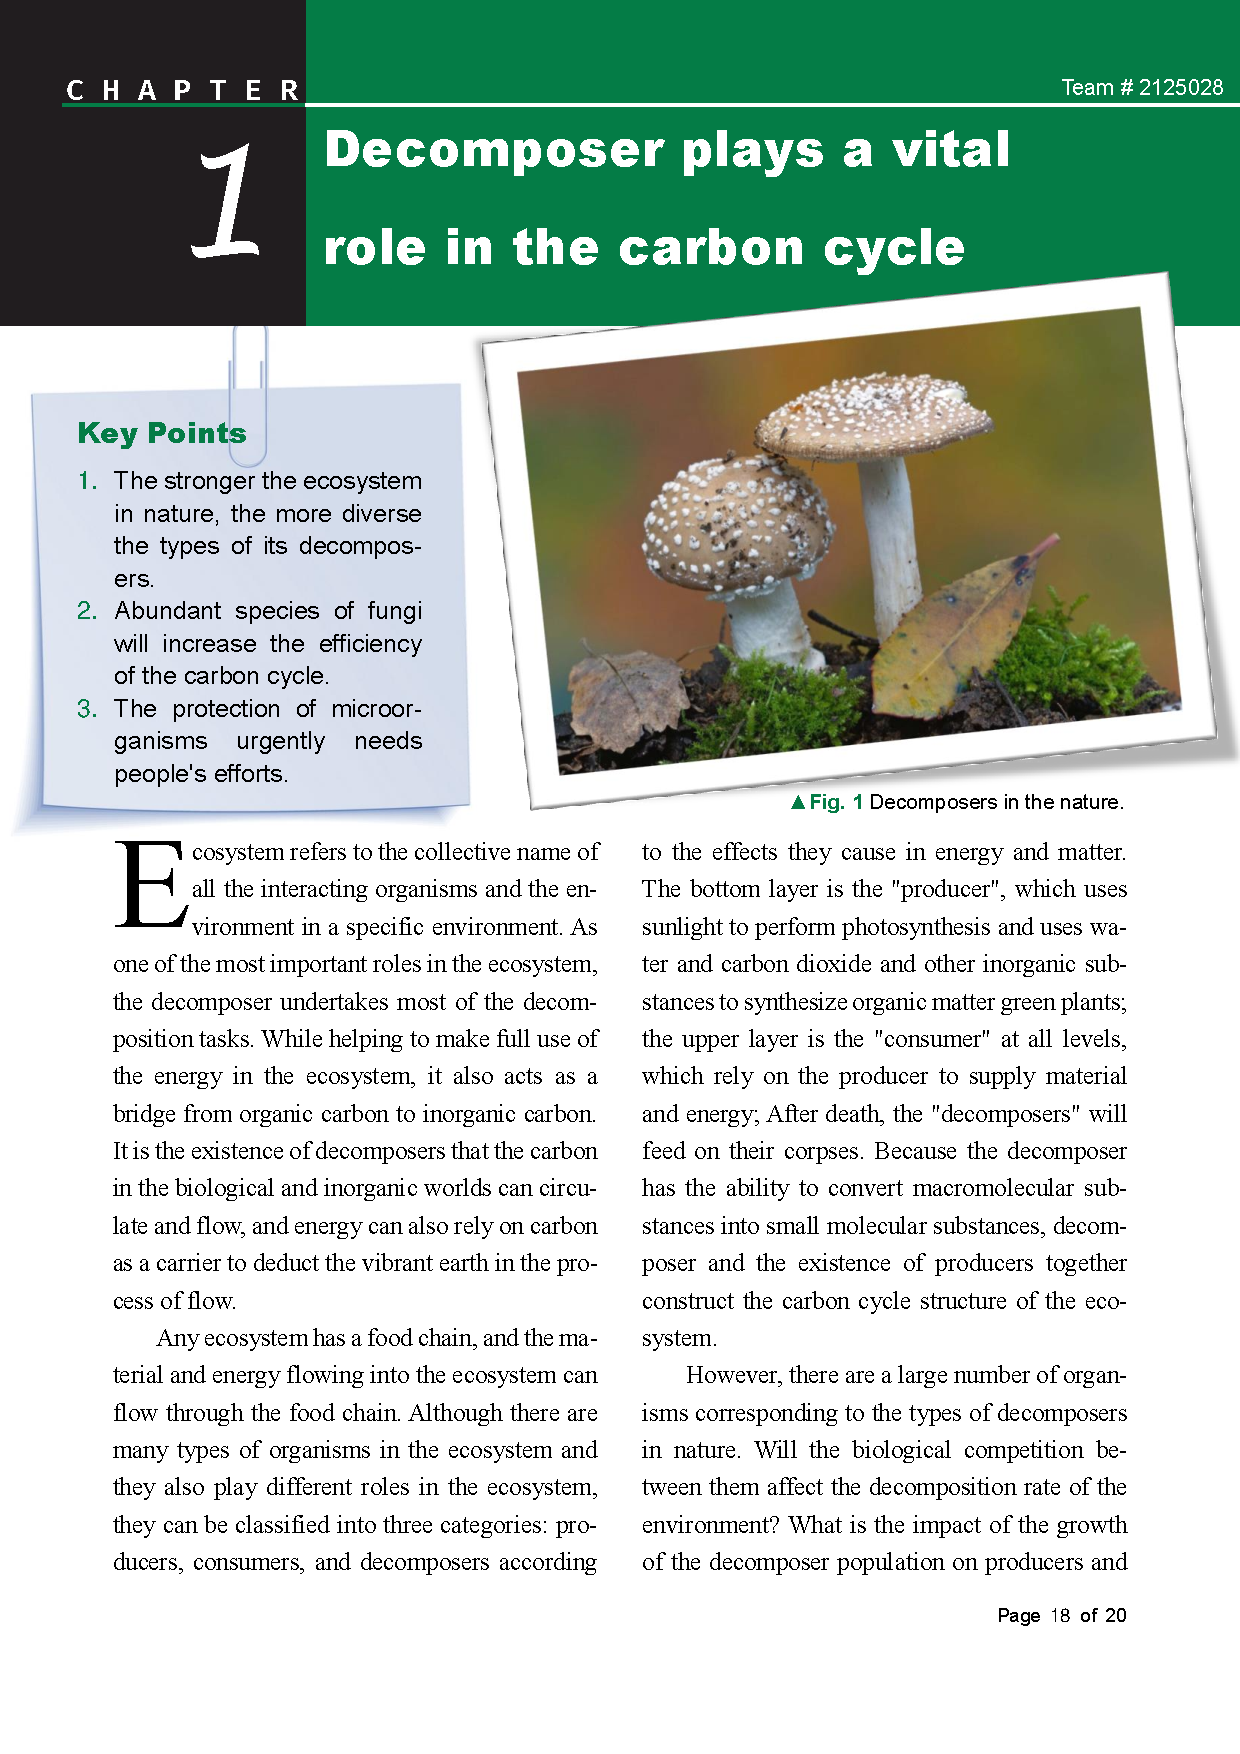
\includepdf[pages=-]{figures/article.pdf}
\newpage
% 第二章
\section{Article for College Level Biology Textbook}
Please turn to the next page.
\newpage
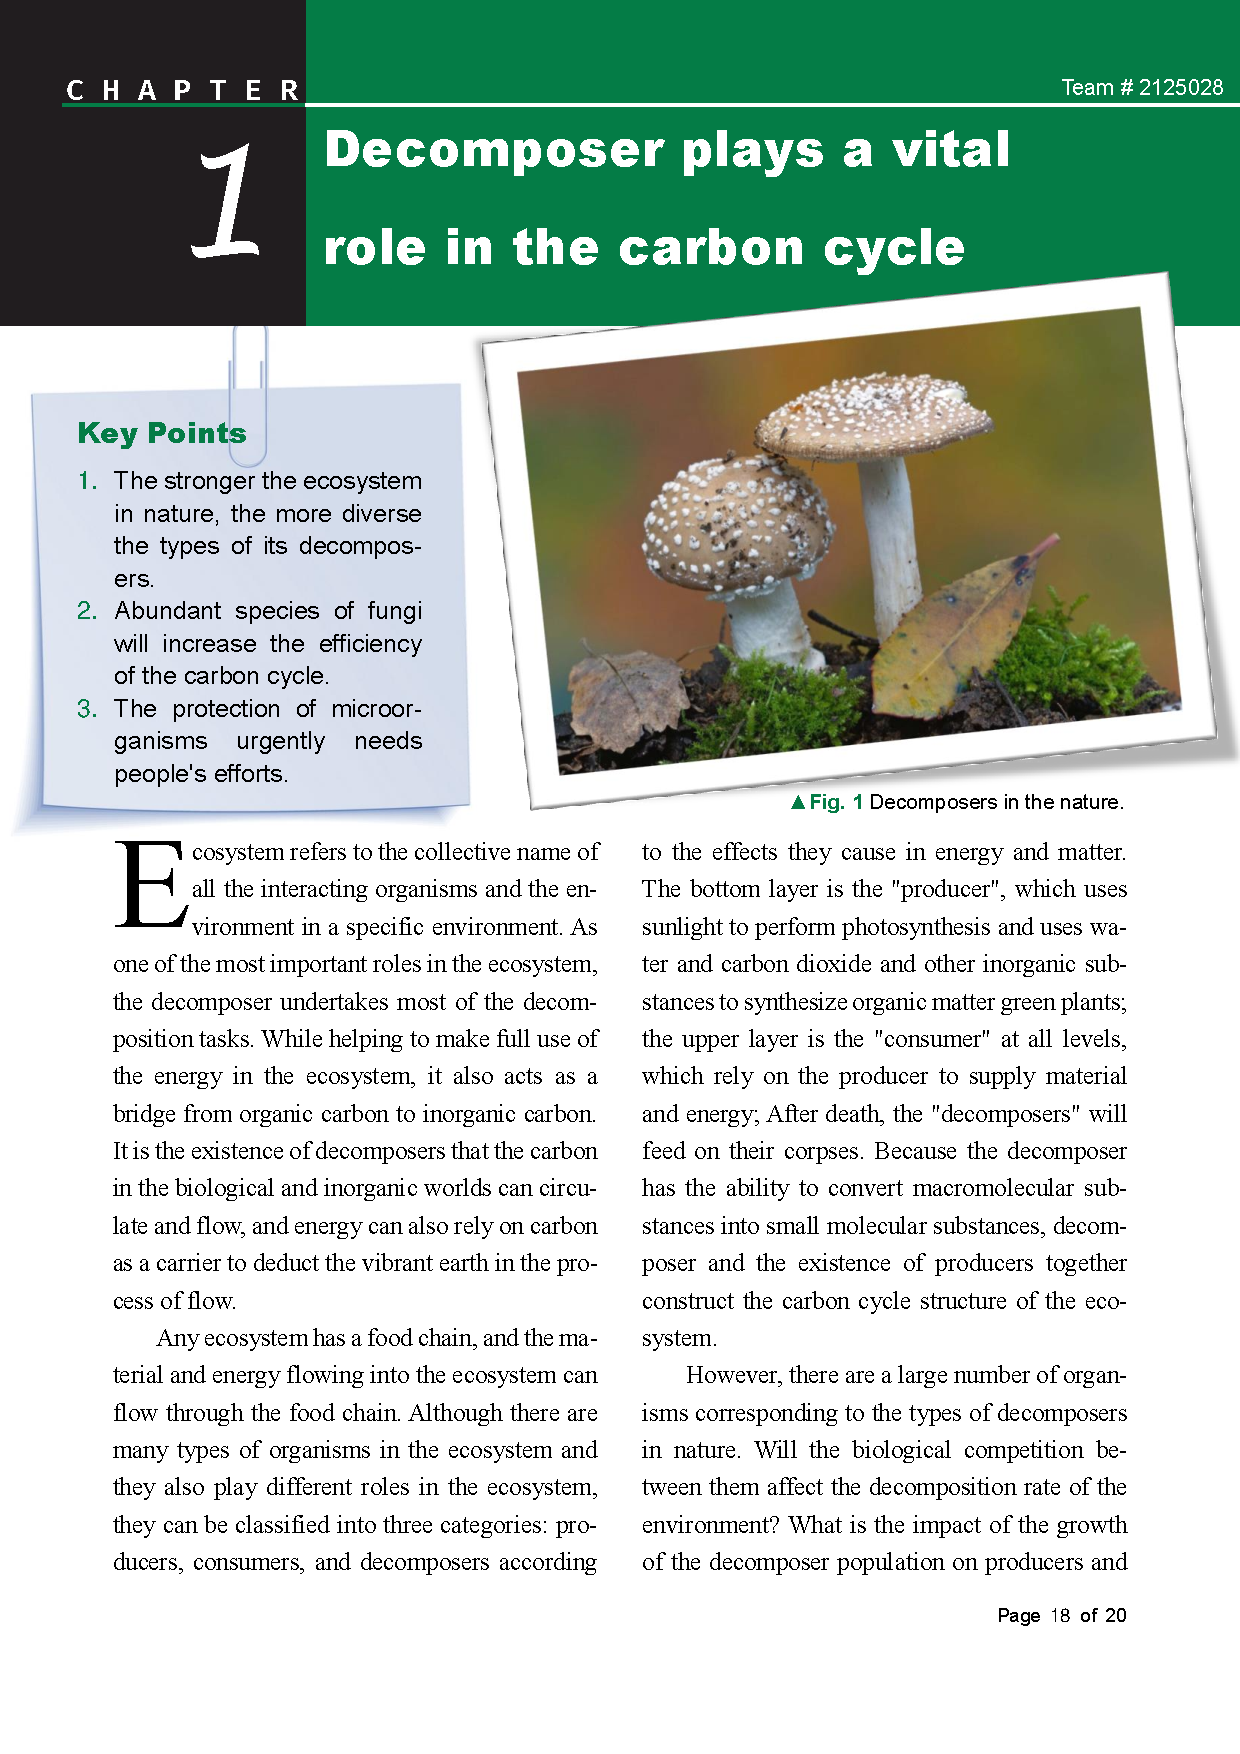
\includepdf[pages=-]{figures/article.pdf}
\newpage
% 第三章
\section{Article for College Level Biology Textbook}
Please turn to the next page.
\newpage
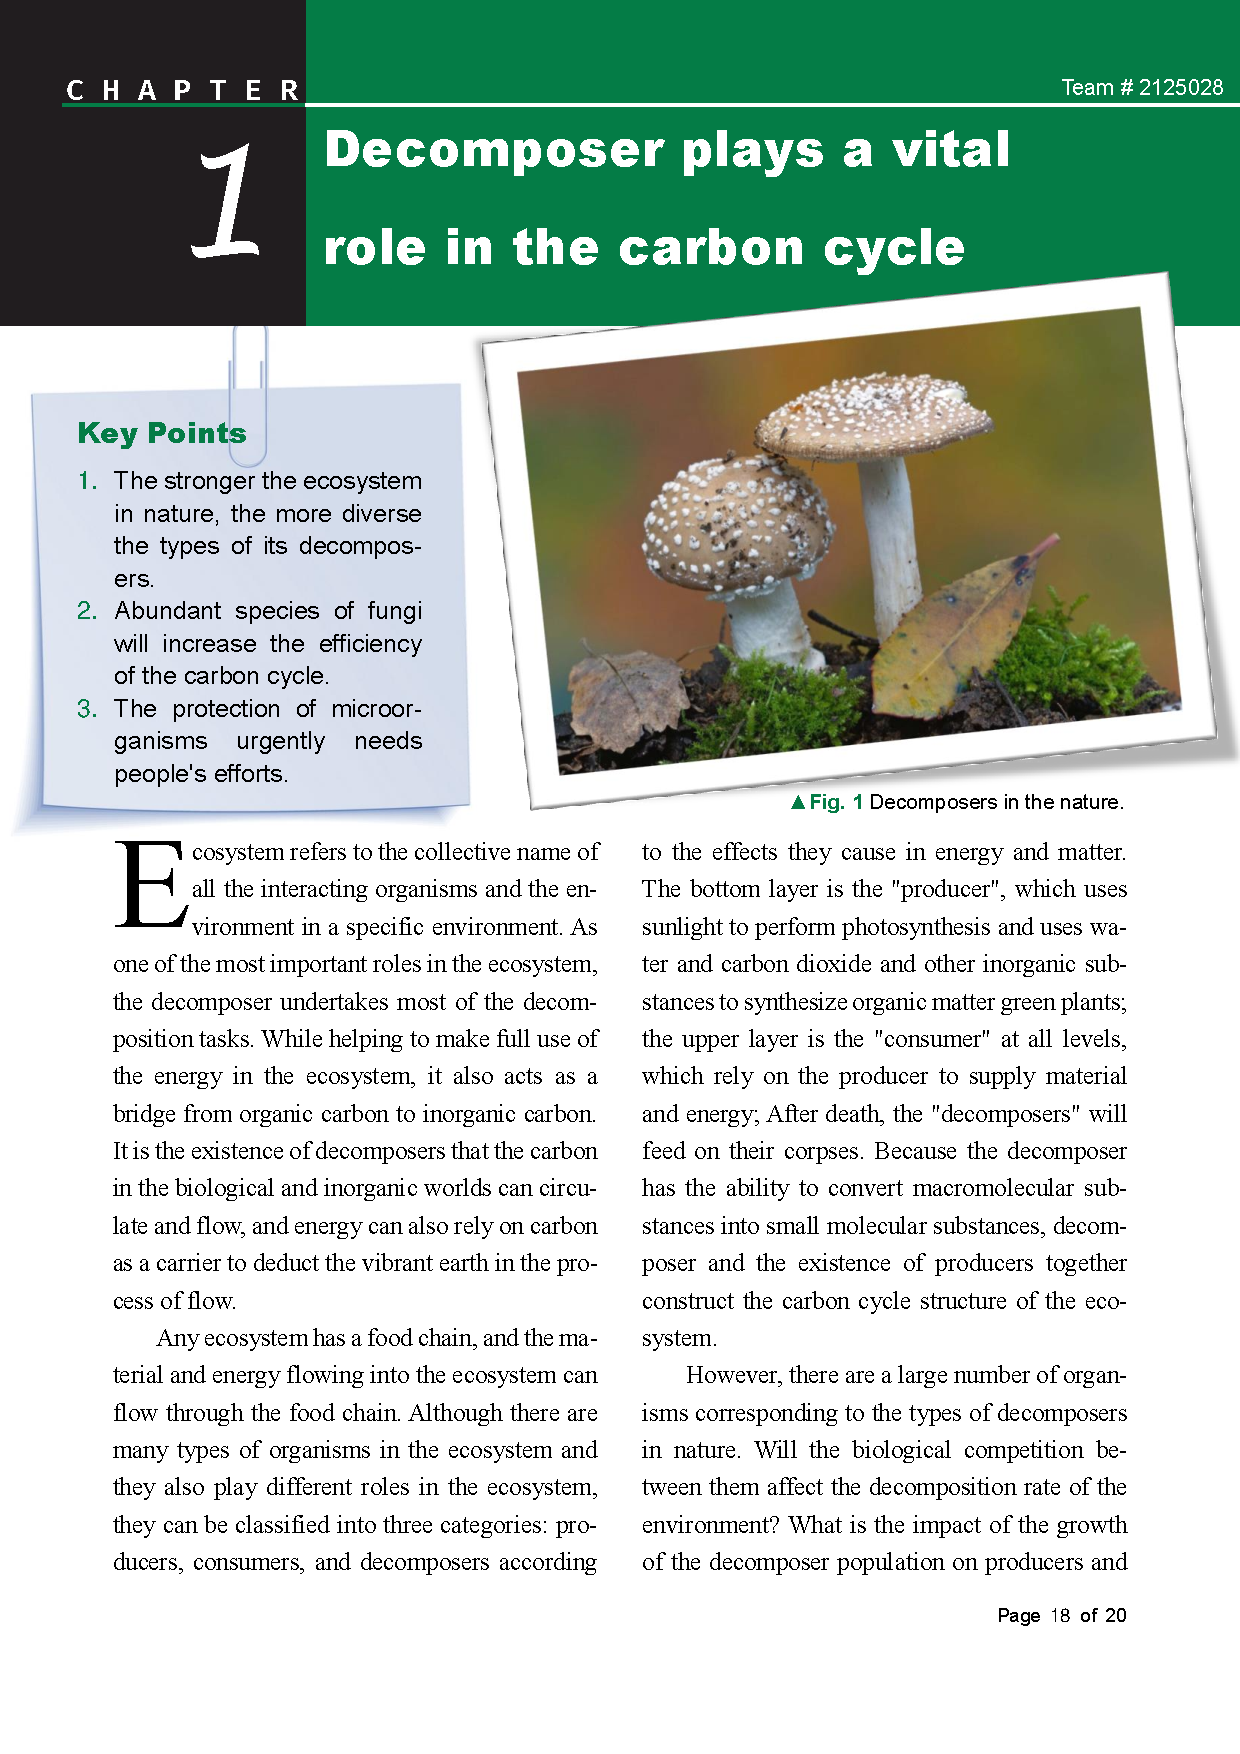
\includepdf[pages=-]{figures/article.pdf}
\newpage
% 第四章
\section{Article for College Level Biology Textbook}
Please turn to the next page.
\newpage
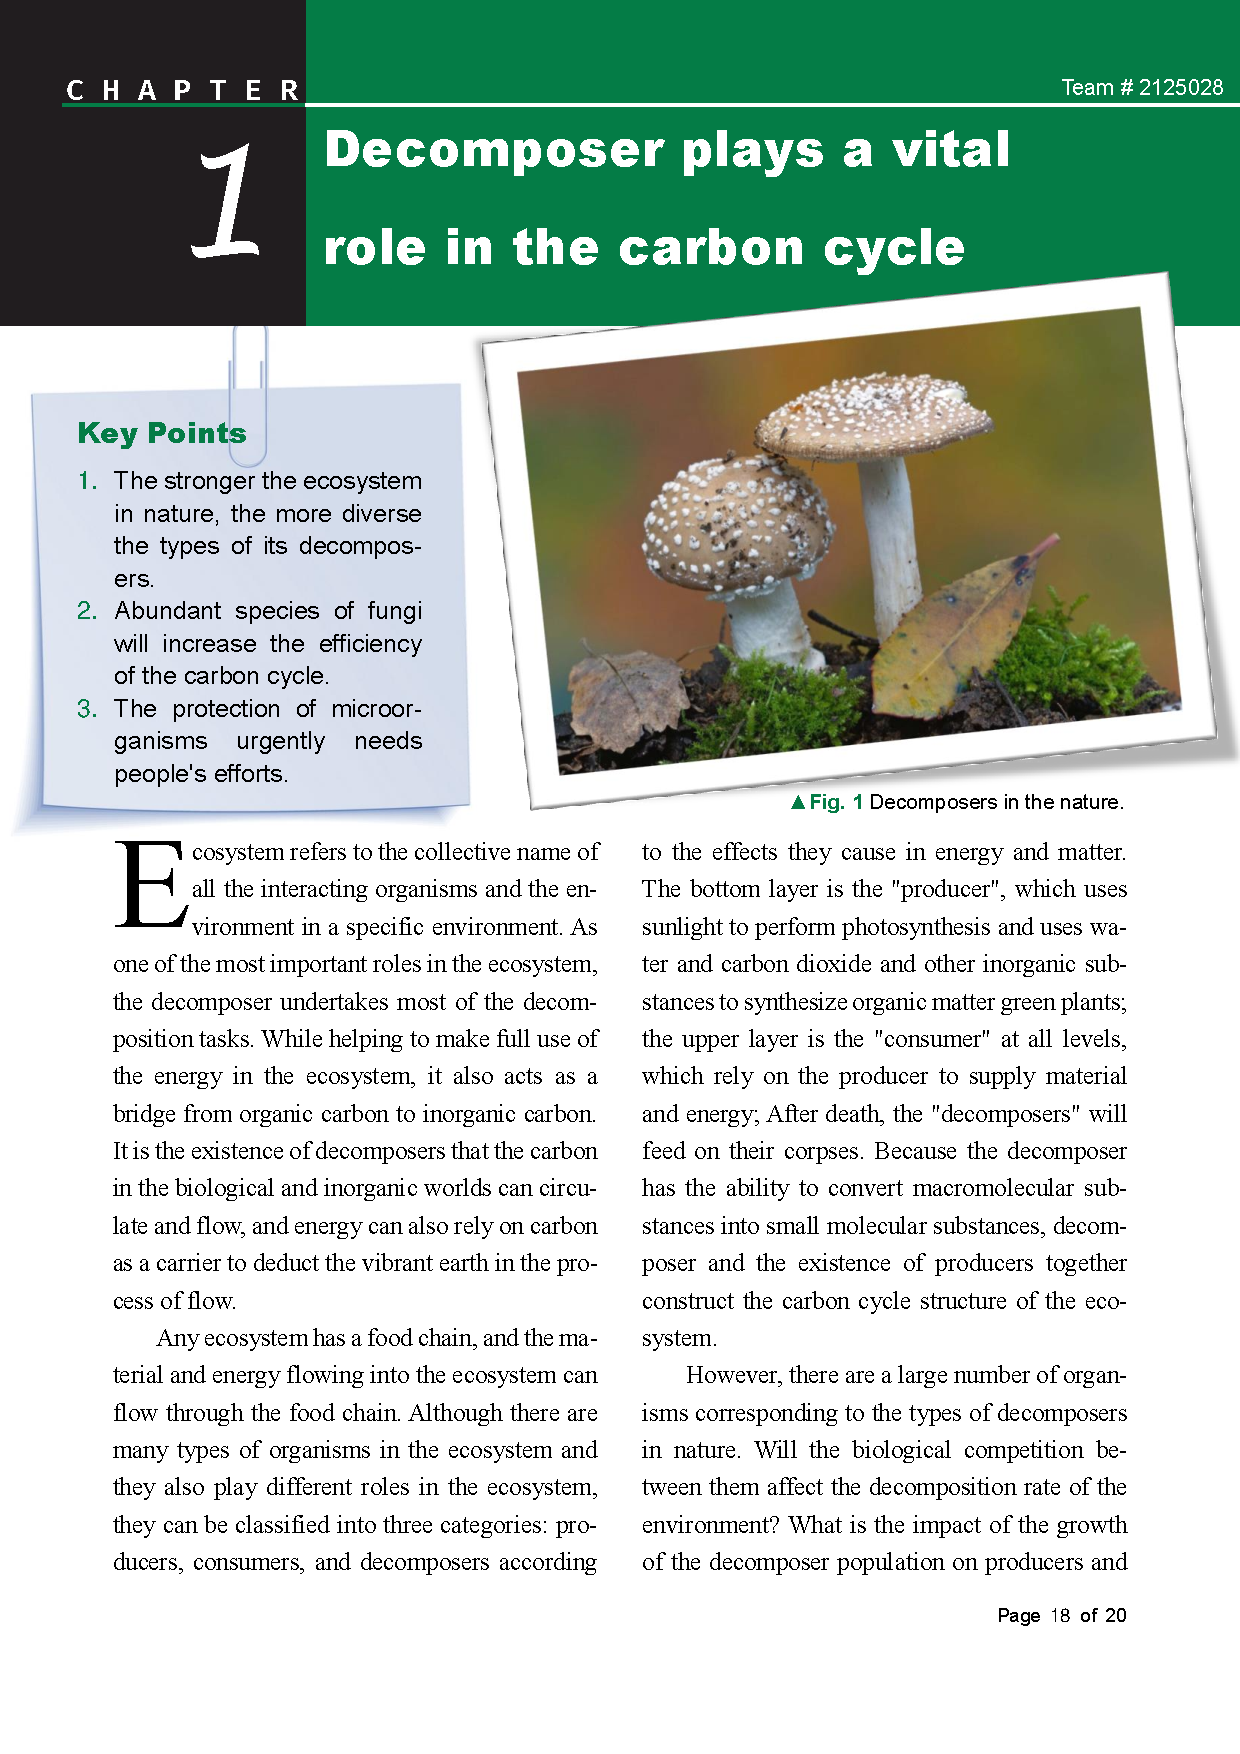
\includepdf[pages=-]{figures/article.pdf}
\newpage
% 第五章
\section{Article for College Level Biology Textbook}
Please turn to the next page.
\newpage
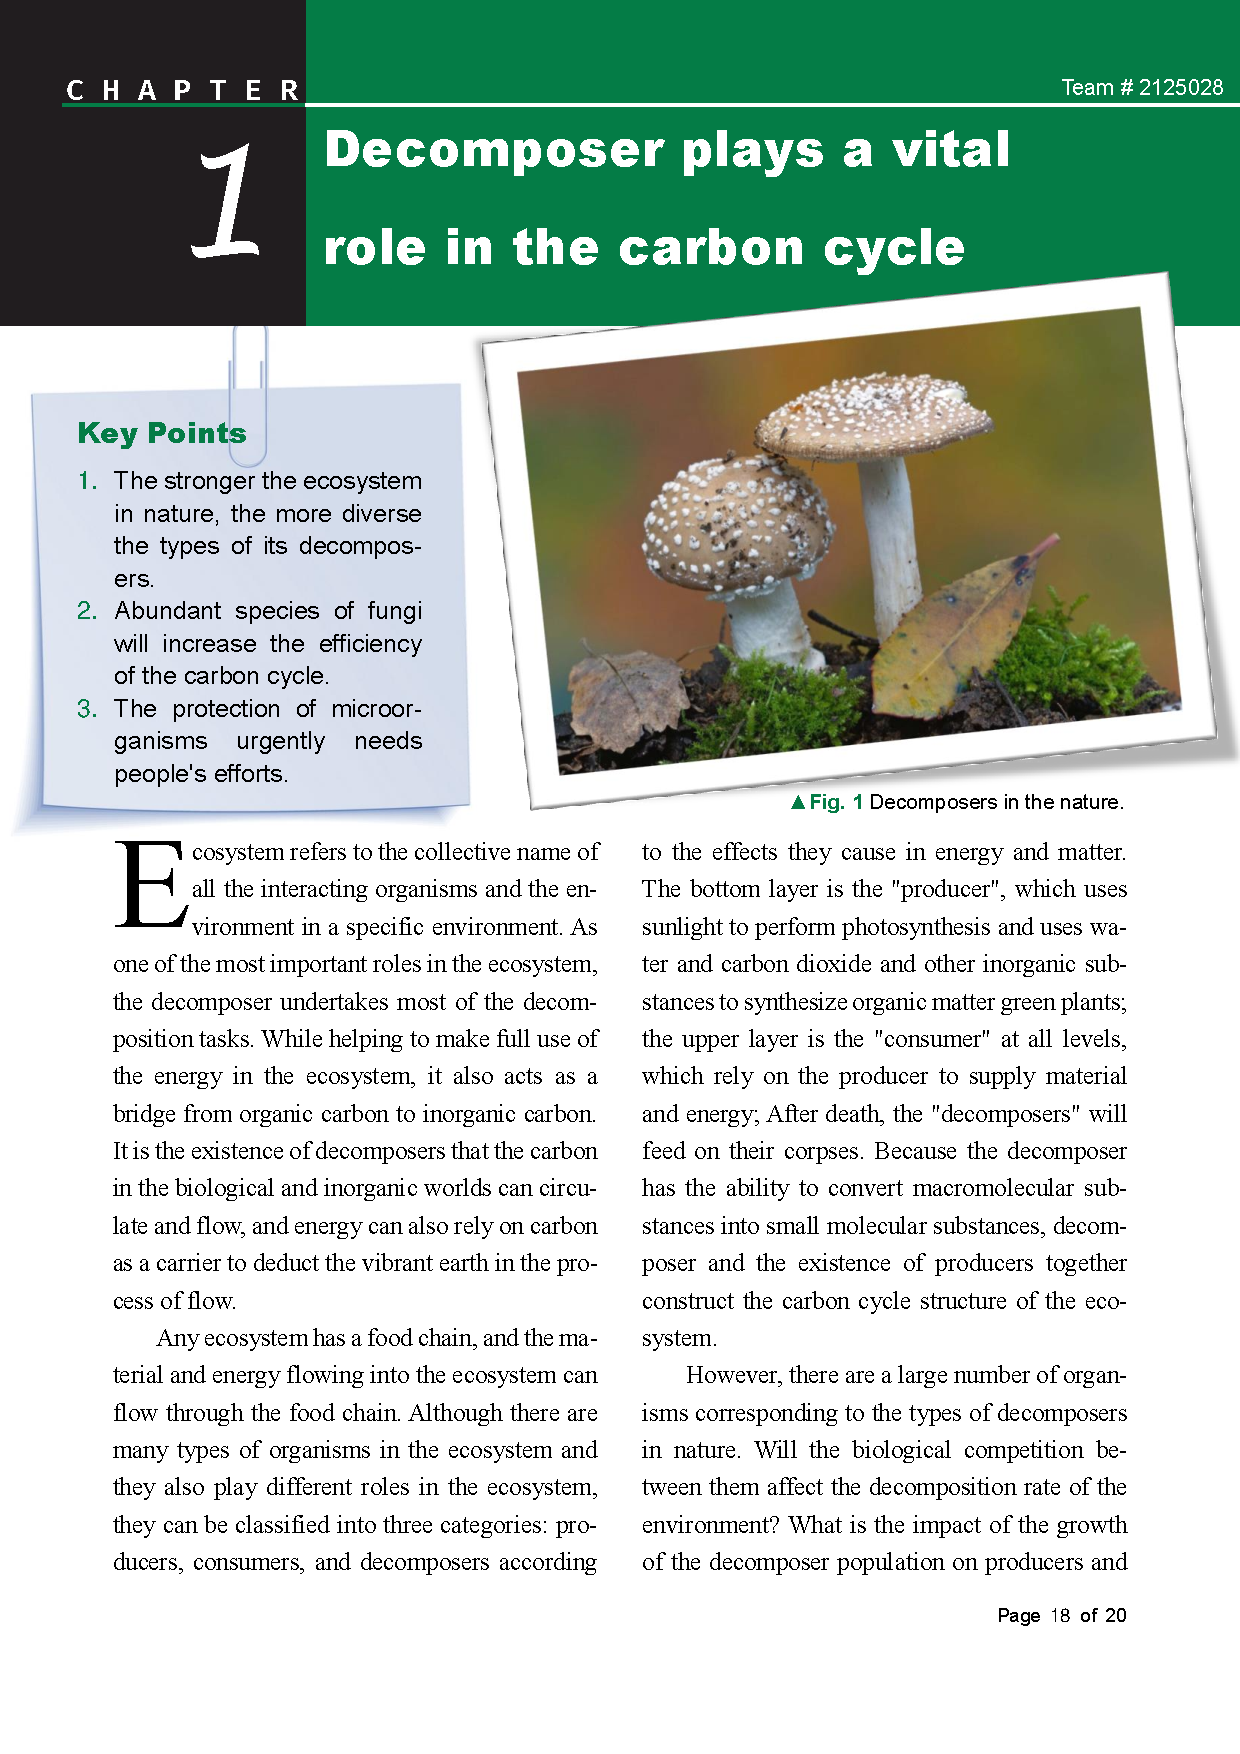
\includepdf[pages=-]{figures/article.pdf}
\newpage
% 第六章
\section{Article for College Level Biology Textbook}
Please turn to the next page.
\newpage
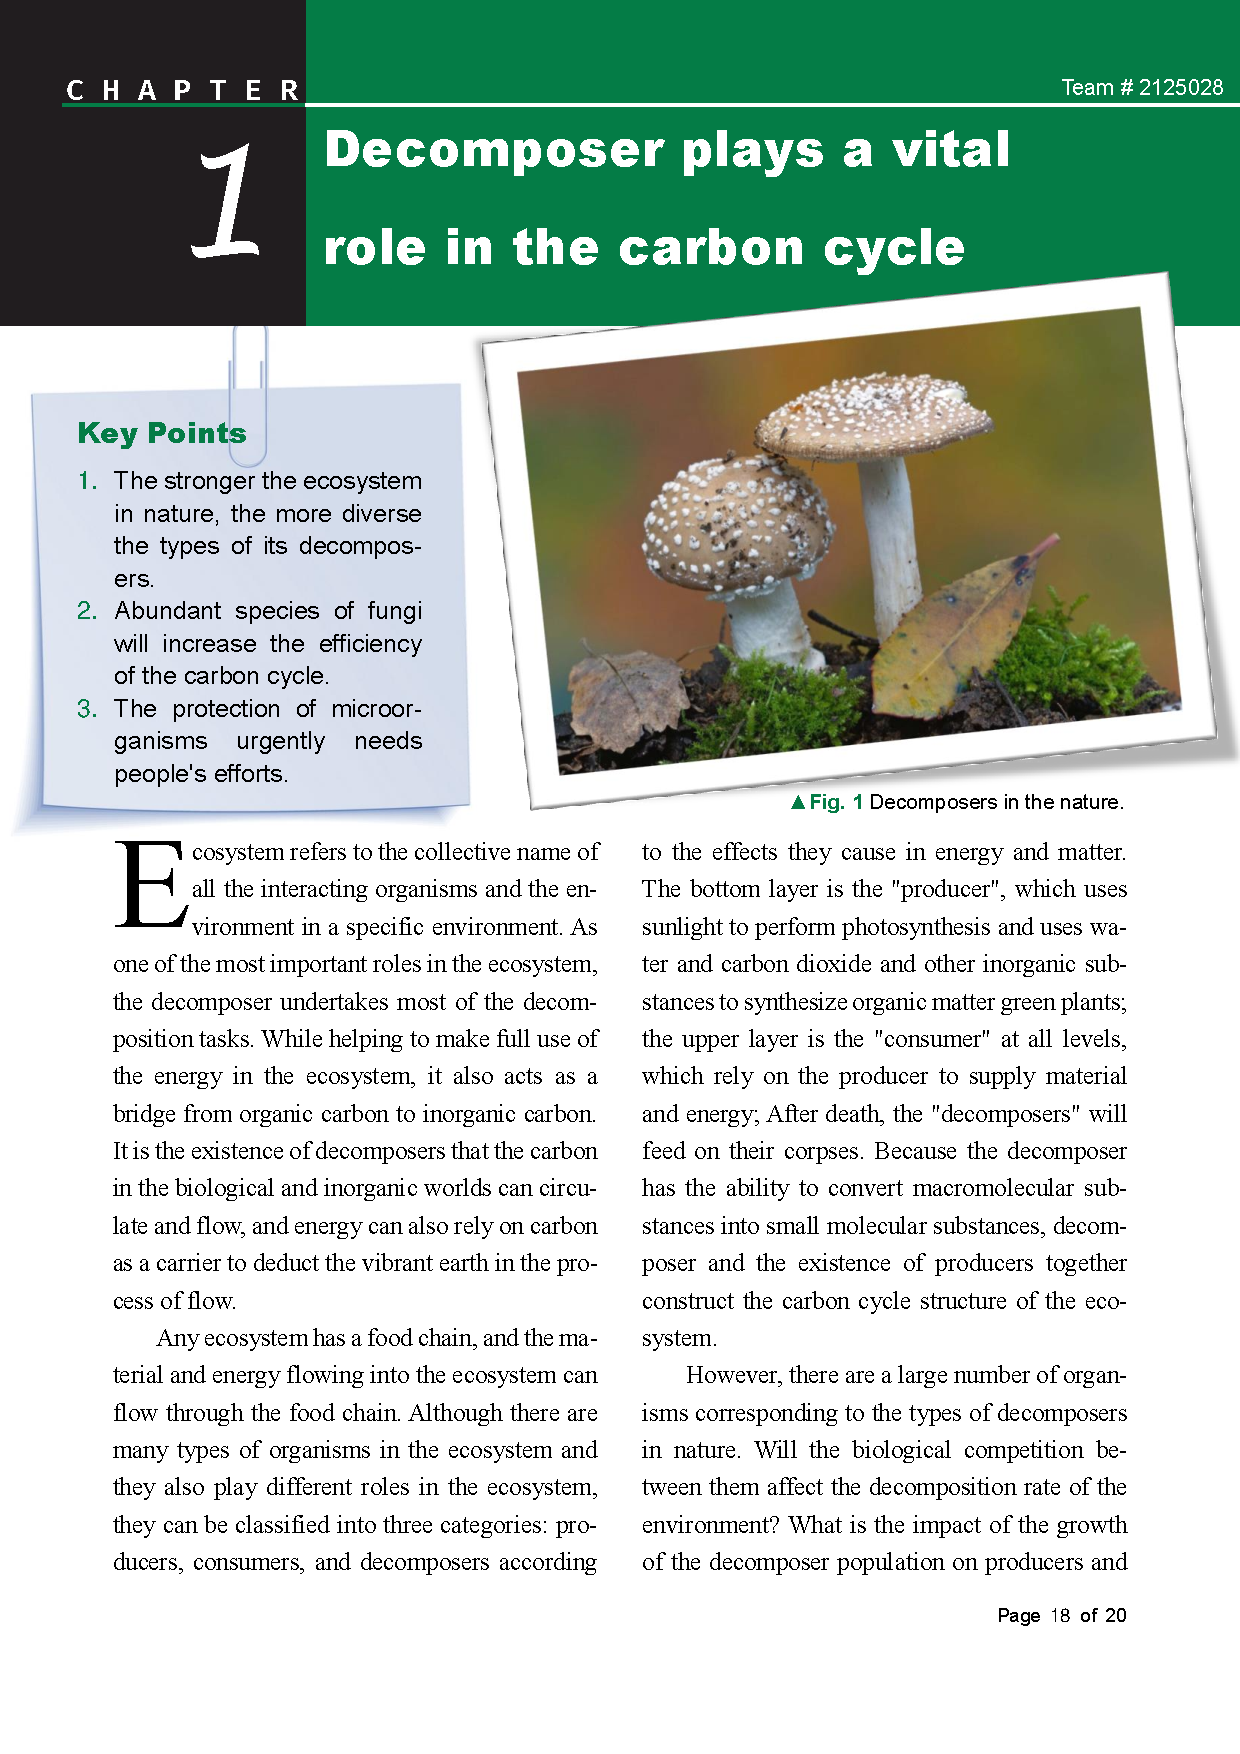
\includepdf[pages=-]{figures/article.pdf}
\newpage
% 第七章
\section{Article for College Level Biology Textbook}
Please turn to the next page.
\newpage
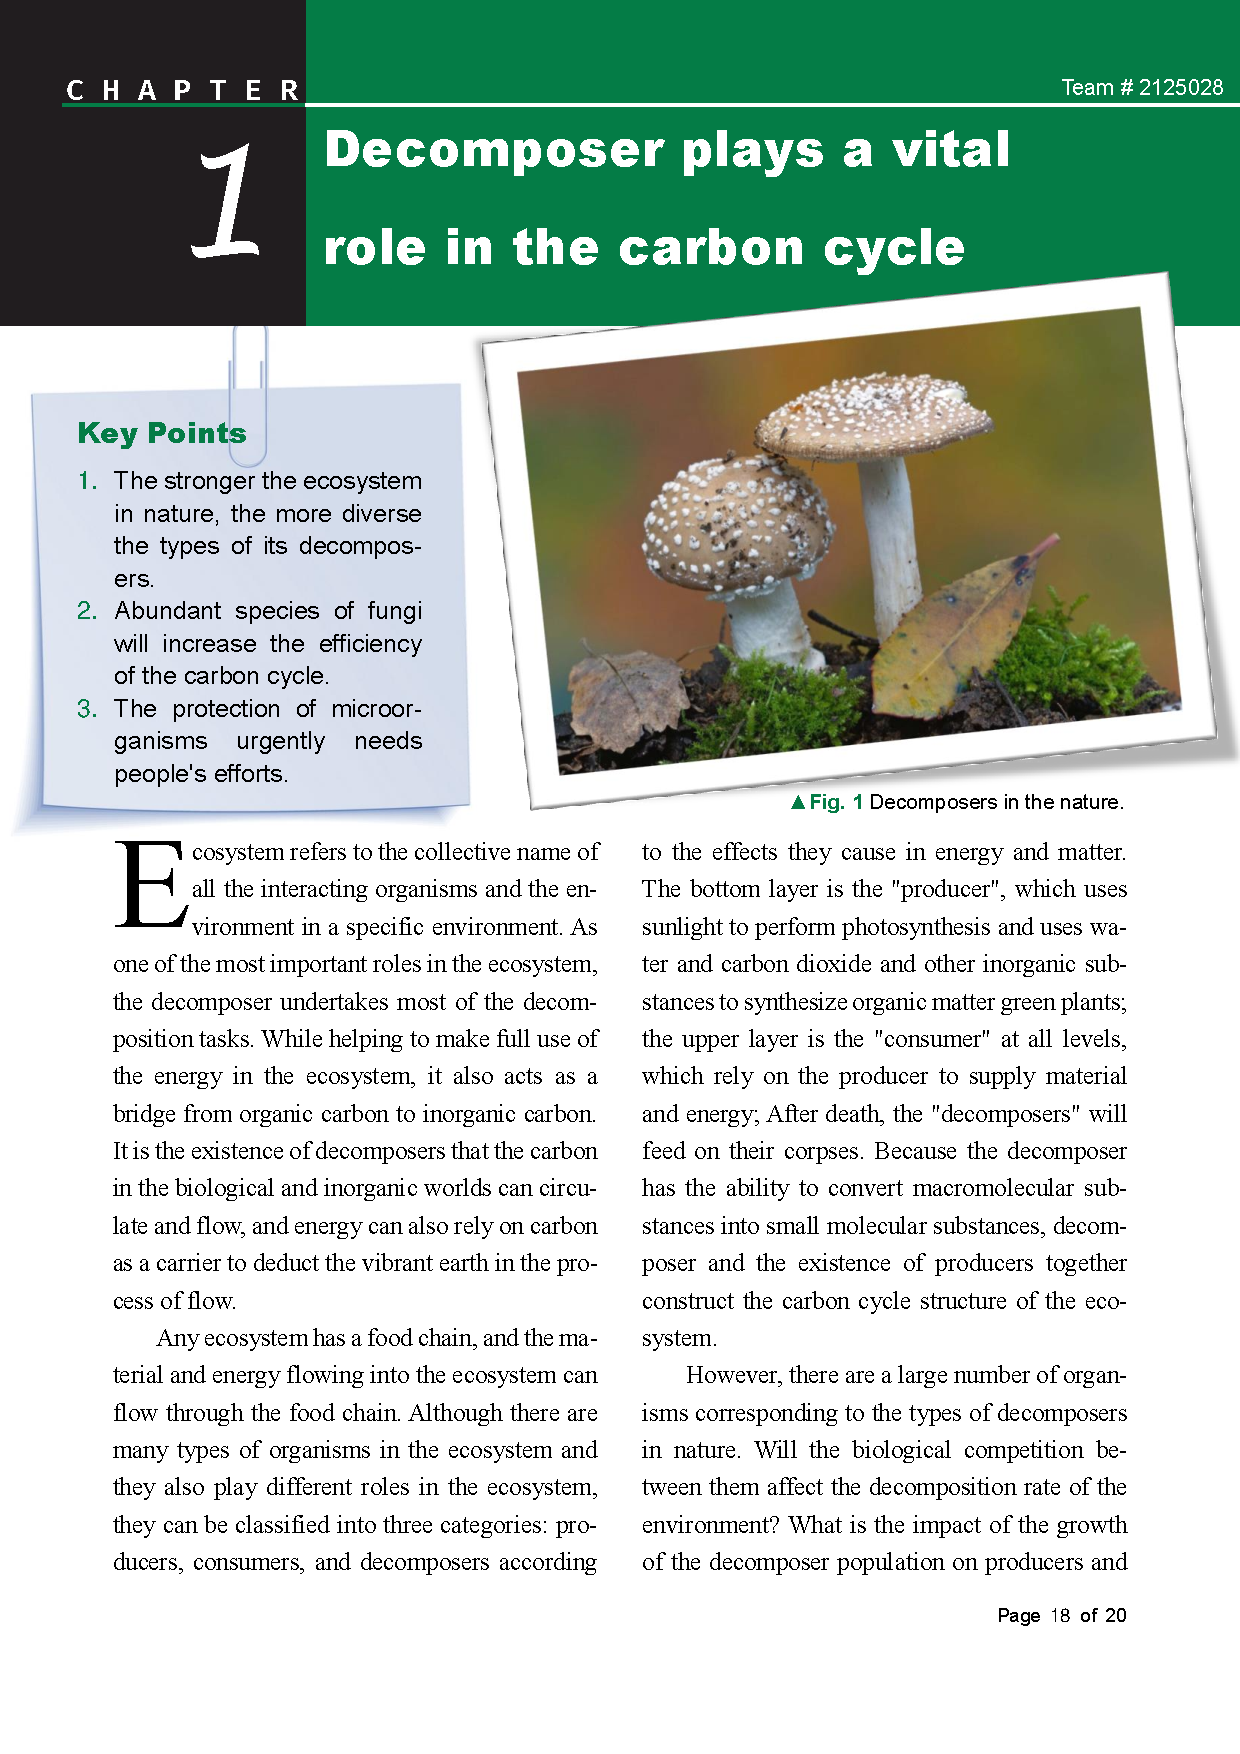
\includepdf[pages=-]{figures/article.pdf}
\newpage
% 参考文献
\section{Article for College Level Biology Textbook}
Please turn to the next page.
\newpage
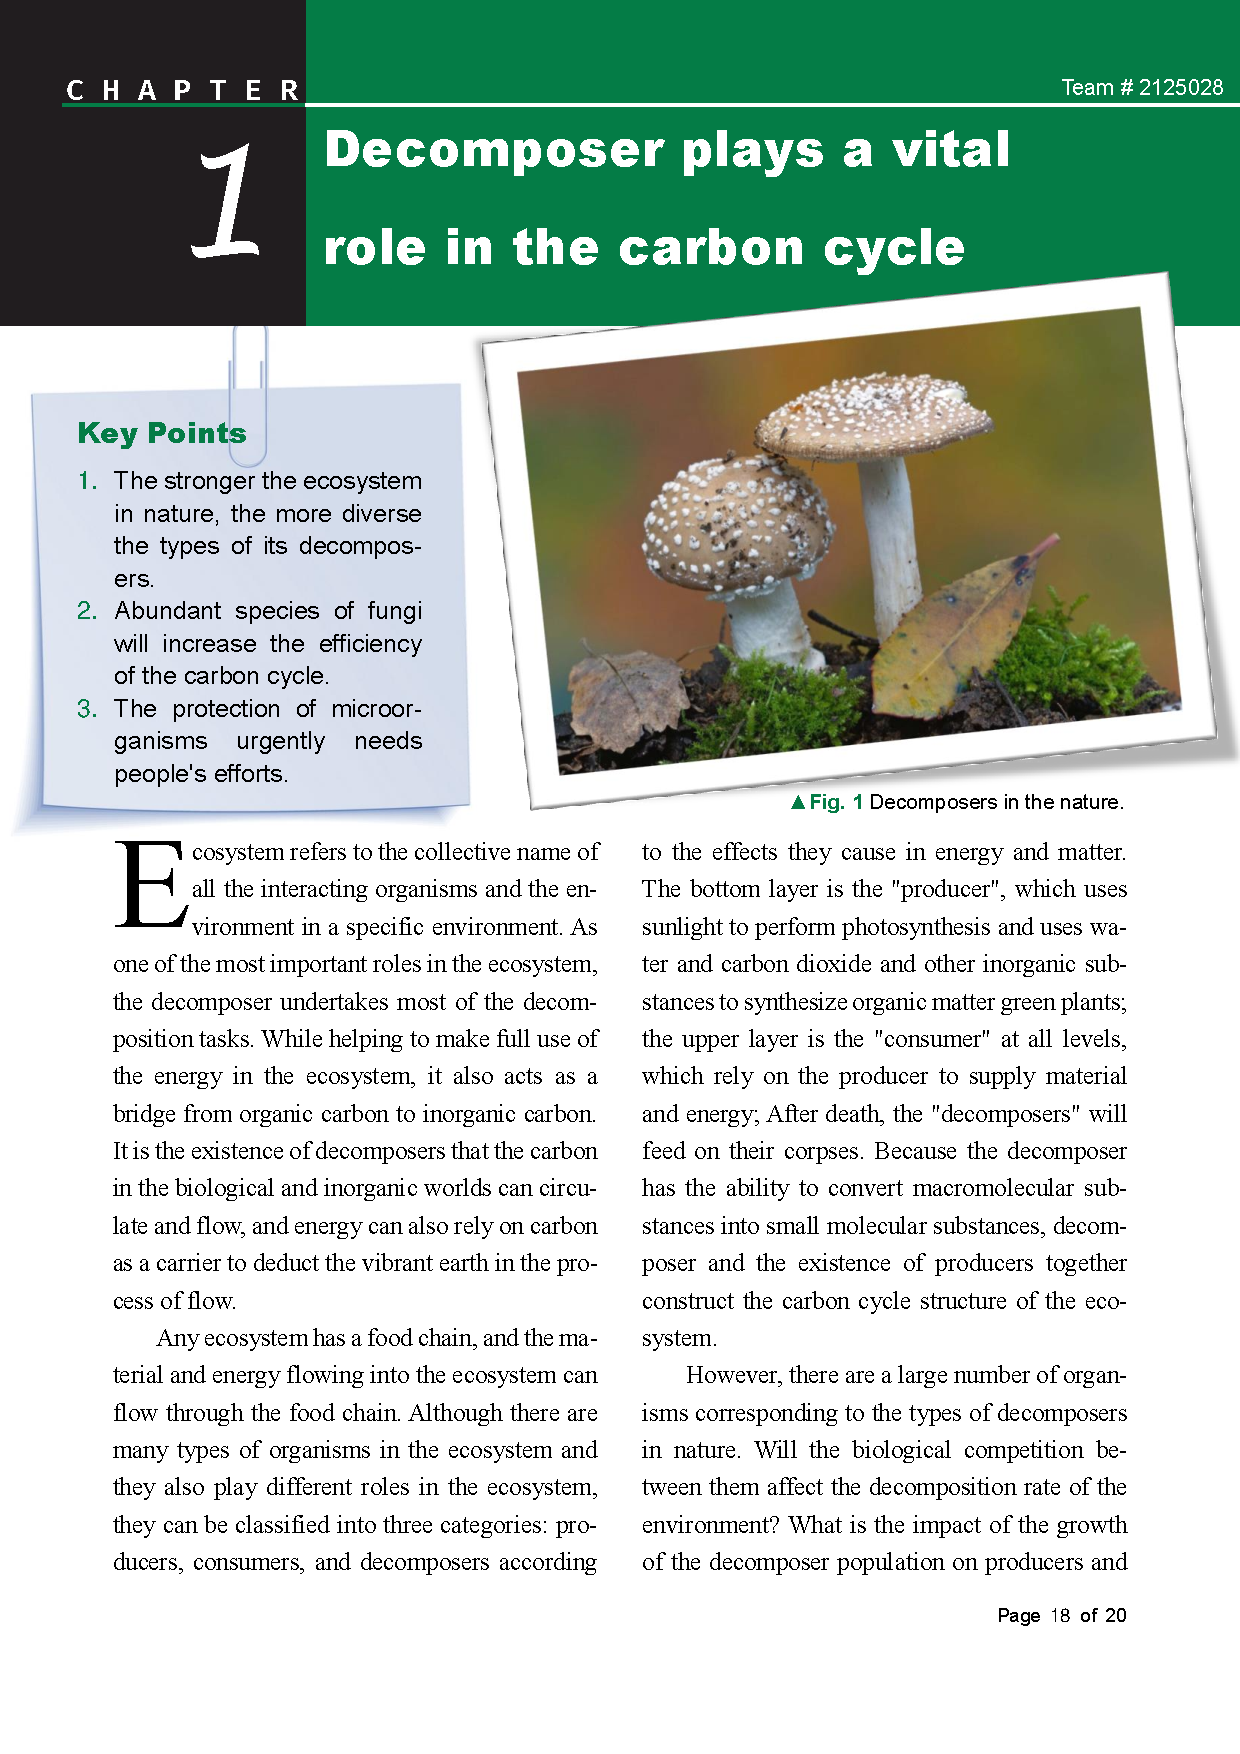
\includepdf[pages=-]{figures/article.pdf}
\newpage
\end{document}
